\documentclass[12pt]{standalone}
\usepackage[utf8]{inputenc}
\usepackage[T1]{fontenc}
\usepackage{times}
\usepackage{amsmath,amssymb}
\usepackage[dvipsnames,svgnames]{xcolor}
\usepackage{tikz}
\usetikzlibrary{decorations.pathreplacing, calc, positioning, shapes.geometric, shapes.symbols, arrows.meta, backgrounds, fit, shapes.misc}
\definecolor{RED}{rgb}{1,0,0}
\definecolor{dmrsfill}{HTML}{CDE2FB}
\definecolor{winblue}{HTML}{0D366B}
\definecolor{inksec}{HTML}{52514E}
\begin{document}
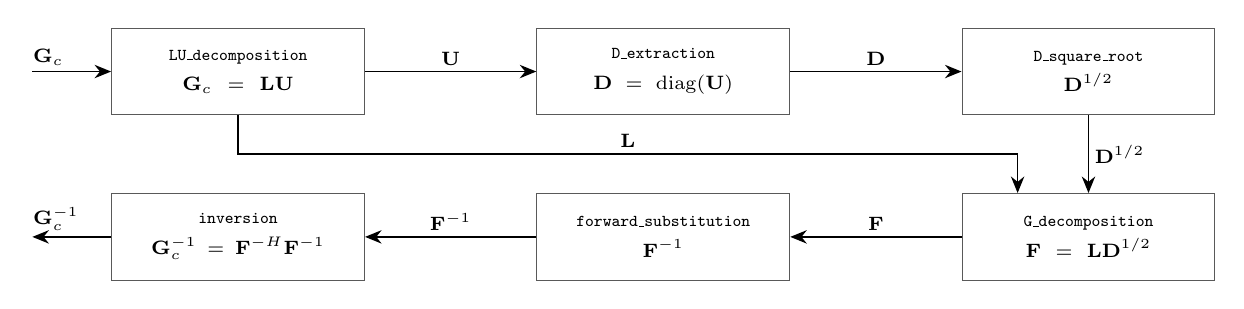
\begin{tikzpicture}[
  font=\fontsize{7.5}{9}\selectfont,
  >={Stealth[length=2.1mm, width=1.7mm]},
  etapa/.style={draw=black!65, fill=white, align=center, text width=3.0cm,
                minimum height=1.1cm, inner sep=3pt},
  seta/.style={->, draw=black, line width=0.6pt},
  rot/.style={font=\fontsize{7}{8.4}\selectfont, inner sep=2pt},
]
% Duas linhas em U: 1 -> 2 -> 3 na linha de cima, desce, 4 -> 5 -> 6 na de baixo.
\newcommand{\fnome}[1]{{\fontsize{6.5}{7.8}\selectfont\ttfamily #1}}
\node[etapa] (e1) at (1.9,0)   {\fnome{LU\_decomposition}\\[2pt] $\mathbf{G}_c = \mathbf{L}\mathbf{U}$};
\node[etapa] (e2) at (7.3,0)   {\fnome{D\_extraction}\\[2pt] $\mathbf{D} = \mathrm{diag}(\mathbf{U})$};
\node[etapa] (e3) at (12.7,0)  {\fnome{D\_square\_root}\\[2pt] $\mathbf{D}^{1/2}$};
\node[etapa] (e4) at (12.7,-2.1) {\fnome{G\_decomposition}\\[2pt] $\mathbf{F} = \mathbf{L}\mathbf{D}^{1/2}$};
\node[etapa] (e5) at (7.3,-2.1)  {\fnome{forward\_substitution}\\[2pt] $\mathbf{F}^{-1}$};
\node[etapa] (e6) at (1.9,-2.1)  {\fnome{inversion}\\[2pt] $\mathbf{G}_c^{-1} = \mathbf{F}^{-H}\mathbf{F}^{-1}$};

\draw[seta] (e1) -- node[rot, above] {$\mathbf{U}$} (e2);
\draw[seta] (e2) -- node[rot, above] {$\mathbf{D}$} (e3);
\draw[seta] (e3) -- node[rot, right] {$\mathbf{D}^{1/2}$} (e4);
\draw[seta] (e4) -- node[rot, above] {$\mathbf{F}$} (e5);
\draw[seta] (e5) -- node[rot, above] {$\mathbf{F}^{-1}$} (e6);
% L vai direto da etapa 1 para a etapa 4, pelo espaço entre as linhas
\path let \p1=(e1.south), \p2=(e4.north), \n1={(\y1+\y2)/2} in
  coordinate (meio) at (0,\n1);
\draw[seta] (e1.south) -- (e1.south |- meio) -- node[rot, above, pos=0.5] {$\mathbf{L}$} ($(e4.north |- meio)+(-0.9,0)$) -- ($(e4.north)+(-0.9,0)$);

% entrada e saída
\draw[seta] (e1.west) ++(-1.0,0) node[rot, above right=0pt and -2pt] {$\mathbf{G}_c$} -- (e1.west);
\draw[seta] (e6.west) -- ++(-1.0,0) node[rot, above right=0pt and -2pt] {$\mathbf{G}_c^{-1}$};
\end{tikzpicture}
\end{document}
